\documentclass{article}
\usepackage[margin=1in]{geometry}
\usepackage[linesnumbered,ruled,vlined]{algorithm2e}
\usepackage{amsfonts}
\usepackage{amsmath}
\usepackage{amssymb}
\usepackage{amsthm}
\usepackage{enumitem}
\usepackage{fancyhdr}
\usepackage{hyperref}
\usepackage{minted}
\usepackage{multicol}
\usepackage{pdfpages}
\usepackage{standalone}
\usepackage[many]{tcolorbox}
\usepackage{tikz-cd}
\usepackage{transparent}
\usepackage{xcolor}
% \tcbuselibrary{minted}

\author{Nathan Solomon}

\newcommand{\fig}[1]{
    \begin{center}
        \includegraphics[width=\textwidth]{#1}
    \end{center}
}

% Math commands
\renewcommand{\d}{\mathrm{d}}
\DeclareMathOperator{\id}{id}
\DeclareMathOperator{\im}{im}
\DeclareMathOperator{\proj}{proj}
\DeclareMathOperator{\Span}{span}
\DeclareMathOperator{\Tr}{Tr}
\DeclareMathOperator{\tr}{tr}
\DeclareMathOperator{\ad}{ad}
\DeclareMathOperator{\ord}{ord}
%%%%%%%%%%%%%%% \DeclareMathOperator{\sgn}{sgn}
\DeclareMathOperator{\Aut}{Aut}
\DeclareMathOperator{\Inn}{Inn}
\DeclareMathOperator{\Out}{Out}
\DeclareMathOperator{\stab}{stab}

\newcommand{\N}{\ensuremath{\mathbb{N}}}
\newcommand{\Z}{\ensuremath{\mathbb{Z}}}
\newcommand{\Q}{\ensuremath{\mathbb{Q}}}
\newcommand{\R}{\ensuremath{\mathbb{R}}}
\newcommand{\C}{\ensuremath{\mathbb{C}}}
\renewcommand{\H}{\ensuremath{\mathbb{H}}}
\newcommand{\F}{\ensuremath{\mathbb{F}}}

\newcommand{\E}{\ensuremath{\mathbb{E}}}
\renewcommand{\P}{\ensuremath{\mathbb{P}}}

\newcommand{\es}{\ensuremath{\varnothing}}
\newcommand{\inv}{\ensuremath{^{-1}}}
\newcommand{\eps}{\ensuremath{\varepsilon}}
\newcommand{\del}{\ensuremath{\partial}}
\renewcommand{\a}{\ensuremath{\alpha}}

\newcommand{\abs}[1]{\ensuremath{\left\lvert #1 \right\rvert}}
\newcommand{\norm}[1]{\ensuremath{\left\lVert #1\right\rVert}}
\newcommand{\mean}[1]{\ensuremath{\left\langle #1 \right\rangle}}
\newcommand{\floor}[1]{\ensuremath{\left\lfloor #1 \right\rfloor}}
\newcommand{\ceil}[1]{\ensuremath{\left\lceil #1 \right\rceil}}
\newcommand{\bra}[1]{\ensuremath{\left\langle #1 \right\rvert}}
\newcommand{\ket}[1]{\ensuremath{\left\lvert #1 \right\rangle}}
\newcommand{\braket}[2]{\ensuremath{\left.\left\langle #1\right\vert #2 \right\rangle}}

\newcommand{\catname}[1]{{\normalfont\textbf{#1}}}

\newcommand{\up}{\ensuremath{\uparrow}}
\newcommand{\down}{\ensuremath{\downarrow}}

% Custom environments
\newtheorem{thm}{Theorem}[section]

\definecolor{probBackgroundColor}{RGB}{250,240,240}
\definecolor{probAccentColor}{RGB}{140,40,0}
\newenvironment{prob}{
    \stepcounter{thm}
    \begin{tcolorbox}[
        boxrule=1pt,
        sharp corners,
        colback=probBackgroundColor,
        colframe=probAccentColor,
        borderline west={4pt}{0pt}{probAccentColor},
        breakable
    ]
    \color{probAccentColor}\textbf{Problem \thethm.} \color{black}
} {
    \end{tcolorbox}
}

\definecolor{exampleBackgroundColor}{RGB}{212,232,246}
\newenvironment{example}{
    \stepcounter{thm}
    \begin{tcolorbox}[
      boxrule=1pt,
      sharp corners,
      colback=exampleBackgroundColor,
      breakable
    ]
    \textbf{Example \thethm.}
} {
    \end{tcolorbox}
}

\definecolor{propBackgroundColor}{RGB}{255,245,220}
\definecolor{propAccentColor}{RGB}{150,100,0}
\newenvironment{prop}{
    \stepcounter{thm}
    \begin{tcolorbox}[
        boxrule=1pt,
        sharp corners,
        colback=propBackgroundColor,
        colframe=propAccentColor,
        breakable
    ]
    \color{propAccentColor}\textbf{Proposition \thethm. }\color{black}
} {
    \end{tcolorbox}
}

\definecolor{thmBackgroundColor}{RGB}{235,225,245}
\definecolor{thmAccentColor}{RGB}{50,0,100}
\renewenvironment{thm}{
    \stepcounter{thm}
    \begin{tcolorbox}[
        boxrule=1pt,
        sharp corners,
        colback=thmBackgroundColor,
        colframe=thmAccentColor,
        breakable
    ]
    \color{thmAccentColor}\textbf{Theorem \thethm. }\color{black}
} {
    \end{tcolorbox}
}

\definecolor{corBackgroundColor}{RGB}{240,250,250}
\definecolor{corAccentColor}{RGB}{50,100,100}
\newenvironment{cor}{
    \stepcounter{thm}
    \begin{tcolorbox}[
        enhanced,
        boxrule=0pt,
        frame hidden,
        sharp corners,
        colback=corBackgroundColor,
        borderline west={4pt}{0pt}{corAccentColor},
        breakable
    ]
    \color{corAccentColor}\textbf{Corollary \thethm. }\color{black}
} {
    \end{tcolorbox}
}

\definecolor{lemBackgroundColor}{RGB}{255,245,235}
\definecolor{lemAccentColor}{RGB}{250,125,0}
\newenvironment{lem}{
    \stepcounter{thm}
    \begin{tcolorbox}[
        enhanced,
        boxrule=0pt,
        frame hidden,
        sharp corners,
        colback=lemBackgroundColor,
        borderline west={4pt}{0pt}{lemAccentColor},
        breakable
    ]
    \color{lemAccentColor}\textbf{Lemma \thethm. }\color{black}
} {
    \end{tcolorbox}
}

\definecolor{proofBackgroundColor}{RGB}{255,255,255}
\definecolor{proofAccentColor}{RGB}{80,80,80}
\renewenvironment{proof}{
    \begin{tcolorbox}[
        enhanced,
        boxrule=1pt,
        sharp corners,
        colback=proofBackgroundColor,
        colframe=proofAccentColor,
        borderline west={4pt}{0pt}{proofAccentColor},
        breakable
    ]
    \color{proofAccentColor}\emph{\textbf{Proof. }}\color{black}
} {
    \qed \end{tcolorbox}
}

\definecolor{noteBackgroundColor}{RGB}{240,250,240}
\definecolor{noteAccentColor}{RGB}{30,130,30}
\newenvironment{note}{
    \begin{tcolorbox}[
        enhanced,
        boxrule=0pt,
        frame hidden,
        sharp corners,
        colback=noteBackgroundColor,
        borderline west={4pt}{0pt}{noteAccentColor},
        breakable
    ]
    \color{noteAccentColor}\textbf{Note. }\color{black}
} {
    \end{tcolorbox}
}


\fancyhf{}
\setlength{\headheight}{24pt}

\date{\today}
\title{MATH 131B Homework \#1}

\begin{document}
\maketitle

\begin{prob}
    Exercises 1.1.13, 1.2.2, 1.2.3, 1.4.7, and 1.5.2 from the textbook
\end{prob}
\textbf{Exercise 1.1.13. Prove Proposition 1.1.19.}
\par
If there exists $N \geq m$ such that $x^{(n)}=x$ for all $n \geq N$, then the distance from $x^{(n)}$ to $x$ in the discrete metric is zero for all $n \geq N$, which means for any $\varepsilon > 0$ and any $n \geq N$, $d(x^{(n)}, x) \leq \varepsilon$, so the sequence converges to $x$.
\par
If the sequence converges to $x$ in the discrete metric, then let $\varepsilon$ be a positive number less than 1. By definition 1.1.14, there exists some $N \geq m$ such that for any $n \geq N$, $d(x^{(n)}, x) \leq \varepsilon < 1$. But in the discrete metric, $d(x^{(n)},x)$ can only be less than one if $x^{(n)}=x$, so for all $n \geq N$, $x^{(n)}=x$.
\bigskip
\par
\textbf{Exercise 1.2.2. Prove Proposition 1.2.10. (Hint: for some of the implications one will need the axiom of choice, as in Lemma 8.4.5.)}
\par
\fbox{($a \Rightarrow b$)} If $x_0$ is an adherent point of $E$, then for every radius $r > 0$, the intersection $B(x_0, r) \cap E \neq 0$, which means $x_0$ is not an exterior point of $E$. Since a boundary point is defined as any point that is not an interior point or an exterior point, $x_0$ must be an interior point or a boundary point.
\par
\fbox{($b \Rightarrow c$)} If $x_0$ is an interior point of $E$, let $x_n=x_0$ for every $n$. This sequence clearly converges to $x_0$.
\par
If $x_0$ is a boundary point of $E$, and we assume the axiom of choice, then for any $n \in \N$, we can define $x_n$ to be some point in $B(x_0, \frac{1}{n}) \cap E$. We know that $B(x_0, \frac{1}{n}) \cap E$ is nonempty because $x_0$ is not an exterior point of $E$, and we know this sequence converges to $x_0$ because $d(x_n, x_0) < \frac{1}{n}$.
\par
\fbox{($c \Rightarrow a$)} Let $x_n$ be a sequence in $E$ which converges to $x_0$. For any $r > 0$, there is some $N$ such that for any $n \geq N$, $d(x_n, x_0) < r$. This means $B(x_0, r)$ contains $\left\{ x_N, x_{N+1}, \dots \right\}$, which are all points in $E$, so $B(x_0, r) \cap E$ is nonempty. Therefore $x_0$ is an adherent point of $E$.
\bigskip
\par
\textbf{Exercise 1.2.3. Prove Proposition 1.2.15. (Hint: you can use earlier parts of the proposition to prove later ones.)}
\begin{enumerate}[label=(\alph*)]
    \item If $E$ is open, then $\partial E \cap E = \emptyset$. Let $x$ be any point in $E$. Then $x \not\in \partial E$. Since $x$ is not in the exterior of $E$ or in the boundary of $E$, it must be in the interior of $E$. Therefore $E$ is a subset of the interior of $E$. But of course, if $x$ is in the interior of $E$, there is some $r>0$ such that $B(x, r) \subset E$, which means $x \in E$. Therefore the interior of $E$ is also a subset of $E$, so $E$ is equal to its own interior.
        \par
        If $E$ is equal to its own interior, then $E \cap \partial E = \operatorname{int}(E) \cap \partial E$. But since the boundary is defined as the points which aren't in the interior or exterior, the boundary and the interior are disjoint, so that intersection is empty, which means $E$ is open.
    \item If $E$ is closed, then $\partial E \subset E$, which means every $x \in E$ is an interior point or a boundary point. By proposition 1.2.10, which we just proved, this means $x$ is an adherent point of $E$.
        \par
        Every boundary point of $E$ is an adherent point (because adherent points are defined as any point not in the exterior, and boundary points are defined as any point not in the exterior or interior). Therefore if $E$ contains all of its adherent points, it must also contain all its boundary points, so $E$ is closed.
    \item Let $x$ be any element of $B(x_0, r)$, and let $r'=(r-d(x_0, x))/2$. Then $B(x, r')$ must be fully contained in $B(x_0, r)$, because for any $x' \in B(x, r')$,
        \[ d(x', x_0) \leq d(x', x) + d(x, x_0) \leq r' + d(x_0, x) = \frac{r+d(x_0,x)}{2} \leq \frac{r+r}{2} = r. \]
        By proposition 1.2.15 part (a), this means $B(x_0, r)$ is open.
        \par
        Suppose $x$ is some point a distance greater than $r$ from $x_0$. Then by the triangle inequality, $B(x, d(x, x_0)-r)$ does not intersect with the closed ball of radius $r$ centered at $x_0$. Therefore $x$ is an exterior point of that closed ball. Every point a distance less than or equal to $r$ away from $x_0$ must then be either an interior point or a boundary point of $ \left\{ x\in X | d(x, x_0) \leq r \right\}$. Since that set contains all of its own boundary points, it is closed.
    \item Take ``any" infinite sequence of points in $ \left\{ x_0 \right\}$ (there is only one such sequence). Every element in that sequence is the same point, so the sequence converges to that point, which is $x_0$. By proposition 1.2.15 part (b), this means $ \left\{ x_0 \right\}$ is closed.
    \item If $E$ is open, then $E \cap \partial E = \emptyset$, which means $\partial E \subset (X \backslash E)$. By the definition of a boundary, the boundary of $E$ is the same as the boundary of $X \backslash E$, so $X \backslash E$ contains all its boundary points, so it is closed.
        \par
        If $X \backslash E$ is closed, then it contains all of its boundary points, so it contains $\partial E$, so $E$ contains none of its boundary points, so $E$ is open.
    \item Let $x$ be any element of $x$. Then there exists some $r_1, \dots, r_n > 0$ such that $B(x, r_1) \subset E_1, \dots, B(x, r_n) \subset E_n$. Let $r$ be the minimum of $ \left\{ r_1, \dots, r_n \right\}$. Then $r>0$ and $B(x, r) \subset E_1 \cap E_2 \cap \cdots \cap E_n$, so that union is open.
        \par
        If $F_1, \dots, F_n$ is a finite collection of closed sets in $X$, then the complement of their union is the intersection of their complements (by De Morgan's law). Their complements are all open, so the intersection of their complements is open, so the complement of their union is open, so their union is closed.
    \item For any $x \in \cup_{\alpha \in I} E_\alpha$, there exists some $\alpha \in I$ such that $x \in E_\alpha$. Since $E_\alpha$ is open, there exists $\varepsilon > 0$ such that $B(x, \varepsilon) \subset E_\alpha$, and that same ball is also contained in the union $\cup_{\alpha \in I} E_\alpha$, so that union is open.
        \par
        If $F_\alpha$ is a collection of closed sets in $X$, then $\cup_{\alpha \in I} (X \backslash F_\alpha)$ is the union of a collection of open sets, so it is open. That means its complement, $\cap_{\alpha \in I} F_\alpha$, is closed.
    \item For any $x \in V$, there exists a ball around $x$ which is contained in $V$, and therefore also contained in $E$, so $x$ is in the interior of $E$. That means $V$ is contained in the interior of $E$.
        \par
        If $E$ is a subset of a closed set $K$, and $x \in E$ is an adherent point, then $x$ is not in the exterior of $E$, which means its not in the exterior of $K$, so it's in $K$. Therefore the closure of $E$ is a subset of $K$.
\end{enumerate}

\textbf{Exercise 1.4.7. Prove Proposition 1.4.12.}
\begin{enumerate}[label=(\alph*)]
    \item Suppose $Y$ is complete, and let $y$ be any boundary point of $Y$. For any $n$, let $y_n$ be any point in $B(y, \frac{1}{n}) \cap Y$. That intersection is nonempty by the definition of a boundary point, and I am assuming the axiom of choice in order to choose a point from each. Then $y_n$ is a Cauchy sequence which clearly converges to $y$, and since $Y$ is complete, that means $y \in Y$. Therefore $Y$ contains all its boundary points, so $Y$ is closed.
    \item Let $y_n$ be a Cauchy sequence in $Y$. Since $X$ is complete, $y_n$ must converge to some $x \in X$. Suppose $x \not\in Y$. Since $Y$ is closed, that means $x$ is not an interior or boundary point of $Y$, so it's an exterior point. The definition of an exterior point is that there exists some $r$ such that $B(x, r) \cap Y = \emptyset$, but since $y_n$ converges to $x$, there must be infinitly many $n$ such that $d(y_n, x) < r$ (for any positive $r$). This is a contradiction, so $x$ (the point that $y_n$ converges to) must be in $Y$, which means $Y$ is complete.
\end{enumerate}

\textbf{Exercise 1.5.2. Prove Proposition 1.5.5. (Hint: prove the completeness and boundedness separately. For both claims, use proof by contradiction. You will need the axiom of choice, as in Lemma 8.4.5.)}
\par
We proved in class that ``compact is equivalent to sequentially compact", meaning in a compact metric space, every sequence has a convergent subsequence. Let $x_n$ be any Cauchy sequence in $X$. Then there exists some subsequence $x_{(i_n)}$ which converges to a point we will call $x$. By the definition of convergence, that means that for any $\varepsilon > 0$, there exists $N$ such that for any $i_n \geq N$, $d(x_{(i_n)}, x) < \frac{\varepsilon}{2}$. By the definition of a Cauchy sequence, for any $\varepsilon > 0$, there exists $M$ such that for any $j, k \geq M$, $d(x_j, x_k) < \frac{\varepsilon}{2}$. Now let $N' = \max(N,M)$. Then for any $m, i_n \geq N'$,
\[ d(x_m, x) \leq d(x_m, x_{(i_n)}) + d(x_{(i_n)}, x) \leq \frac{\varepsilon}{2} + \frac{\varepsilon}{2} = \varepsilon, \]
so $x_m$ converges to $x$, which means \fbox{$X$ is complete}.
\par
Let $x$ be any point in $X$, and cover $X$ with infinitely many open balls centered at $x$:
\[ \left\{ B(x, 1), B(x, 2), B(x, 3), \dots \right\}. \]
Since $X$ is compact, there exists a finite subset of that cover which still covers $X$, and for any such finite subcover, we can define $r$ to be the radius of the largest ball in the subcover. By the triangle inequality, since no point in $X$ can be a distance greater than $r$ from $x$, no two points in $X$ can be a distance greater than $2r$ apart, so \fbox{$X$ is bounded}.

\begin{prob}
    Let $(X,d)$ be a metric space and $E \subset X$ a subset.
    \begin{enumerate}[label=(\alph*)]
        \item Show that if $E$ is a finite set, then $E$ is compact.
        \item Suppose in addition that $d=d_{disc}$ is the discrete metric. Show that if $E$ is compact, then $E$ is a finite set.
    \end{enumerate}
\end{prob}
\par
\begin{enumerate}[label=(\alph*)]
    \item Let $ \left\{ a_n \right\}_{n \in \N}$ be any sequence of elements of $E$. By the pigeonhole principle, since $E$ is finite and $ \{a_n\}$ is infinite, there must be some $e \in E$ such that $e$ occurs infinitely many times in $\{a_n\}$. That forms a convergent subsequence of $\{a_n\}$, so $E$ is sequentially compact, which means $E$ is also compact (we proved in class that for metric spaces, sequentially compact is equivalent to compact).
    \item Cover $E$ with singleton sets, which are open in the discrete metric. If $E$ is compact, then it can be covered by finitely many of those singleton sets, which means $E$ has finitely many elements.
\end{enumerate}

\begin{prob}
    Give the following examples.
    \begin{enumerate}[label=(\alph*)]
        \item Find a metric space $(X,d)$ and an infinite collection of open subsets $ \left\{ U_n \right\}_{n \in \N}$ of $X$ such that $\cap_{n \in \N} U_n$ is not open.
        \item Find a metric space $(X, d)$ and an infinite collection of closed subsets $ \left\{ K_n \right\}_{n \in \N}$ of $X$ such that $\cup_{n \in \N} K_n$ is not closed.
    \end{enumerate}
\end{prob}

For both (a) and (b), let $(X, d)$ be $\R$ with the Euclidean metric.
\begin{enumerate}[label=(\alph*)]
    \item Let $U_n = \left( 0, 1 + \frac{1}{n} \right) $. Then $\cap_{n \in \N} U_n = (0, 1]$. Every $U_n$ is open, but $(0, 1]$ is not open.
    \item Let $K_n = \left[ 0, 1 - \frac{1}{n} \right]$. Then $\cup_{n \in \N} = [0, 1)$. Every $K_n$ is closed, but $[0, 1)$ is not closed.
\end{enumerate}

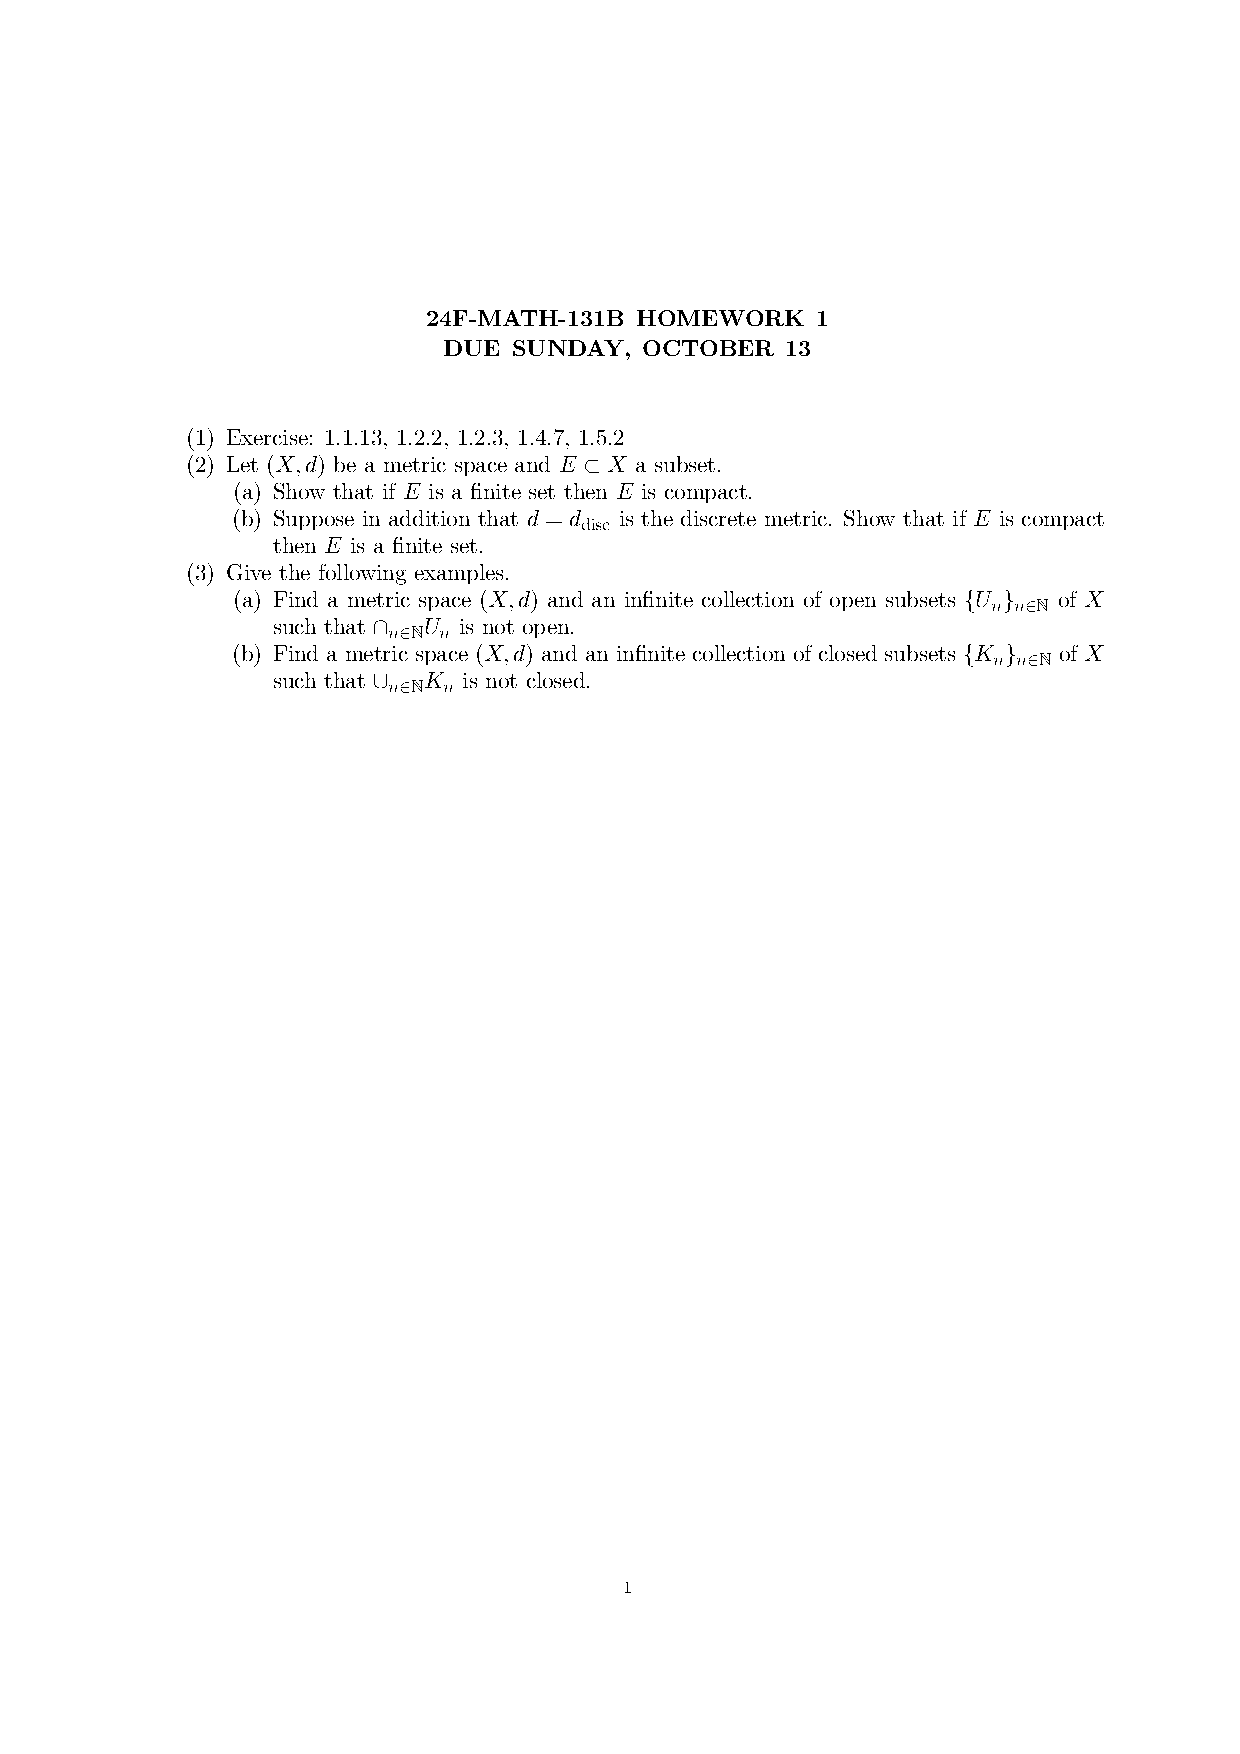
\includepdf[pages=-]{assignment.pdf}

\end{document}
